\subsection{Scattered Light}
\label{s:IDC:scatter}
The sensitivity required to make gravitational wave measurements can
be expressed also as a sensitivity to optical \textit{phase} fluctuations.
The current state of the art is approximately
$10^{-11}$ radians/$\sqrt{\rm Hz}$ and is nominally limited by
quantum mechanics and the available laser power
(cf.~Chapter~\ref{SQN}).
Practically, however, all of the high
sensitivity interferometers in the past 30 years have been limited
at some frequencies by the non-fundamental phase fluctuations due to
scattered light. This phenomenon of excess phase noise due to scattered
light has been known about for decades~\cite{Schilling:1981} but
the methods by which to combat it have been developing steadily since
then and involve the highest levels of experimental artistry in the
field of laser interferometry.

Due to imperfections in the optics, for example, a small fraction of
the laser light escapes from the main interferometer beam path. This
light then interacts with something (e.g. a piece of the vacuum system
or some other suspended optic or beam dump) and then recombines with the
circulating laser field within the
interferometer~\cite{Kip:Scatter95, Kip:scatter1989, Sam:Scatter2012,
Stefano:Scatter, vinet1997scattered, fritschel1998high}.
The recombination may occur at virtually any point within the system:
inside of the Fabry-Perot arm cavities, at the beamsplitter, or even at
the final photodetector which records the GW strain signal. Scattered
light induced phase noise in the sensing of auxiliary degrees of
freedom (cf.~Chapter~\ref{LSC, NFN}) can couple into the strain channel
through the relevant feedback control systems .

It is illuminating to consider \emph{quantitatively} the amplitude of
the noise for a few of these cases.

\subsubsection{Case I: The Beam Tube Baffles}
% based on T1300354
The case of scattering from the multi-km beam tubes connecting the ends of the
interferometer has been studied by Whitcomb, Weiss, Thorne, and Flanagan (for LIGO)
and by Braccini, Vinet, et al. (for Virgo); see references above. Here we provide
a condensed version of their arguments so as to construct a noise budget for backscatter.
Let us assume in this case that the field scatters from the test mass surface,
reflects from a piece of multi-km long beamtube, returns to the same test mass
mirror, and then recombines into the circulating cavity mode. The resulting
phase fluctuation of the electric field will be
\begin{equation}
\delta u_{s} = \frac{4 \pi}{\lambda} x_{s}(f) \sqrt{P_s}
\end{equation}
For comparison, the field fluctuation due to mirror motion will be
\begin{equation}
\delta u_{m} = \frac{4 \pi}{\lambda} x_{m}(f) \sqrt{P_0}
\end{equation}
where $x_s$ is the motion of the beamtube in the direction of the mirror, $x_m$
is the motion of the interferometer mirror, $\lambda$ is the laser wavelength,
$P_0$ is the power stored in the arm cavity, and $P_s$ is the power which
recombines into the circulating cavity mode. Ignoring for a moment the radiation
pressure effects, we can see that the phase noise due to this type of backscatter
can be simply expressed (in units of mirror displacement) using the ratios of
the stored power and the backscattered power which recombines with the cavity mode:
\begin{equation}
x_{m}(f) = x_{s}(f) \sqrt{\frac{P_s}{2 P_0}}
\end{equation}
where the factor of 2 comes from only including phase fluctuations of the backscattered field.

So in order to estimate the $x_m$, we will have to compute $P_s$.
This can be written down by tracing the path of the beam and considering
the relevant scattering cross sections at each step:
\begin{enumerate}
\item The probability for the main beam to scatter into some angle towards a potential backscatterer.
\item The probability for that backscatterer to scatter light back towards the mirror.
\item The probability for that field to scatter back into the cavity mode.
\end{enumerate}
\begin{equation}
P_s = P_0 \frac{\lambda^2}{r^2} \delta \Omega_{ms} \frac{dP}{d\Omega_{ms}} \frac{dP}{d\Omega_{bm}} \frac{dP}{d\Omega_{sm}}
\label{eq:ScatProb1}
\end{equation}
In the above equation, the scatter probability is used; this is related to the
more commonly used Bidirectional Reflectance Distribution Function (BRDF) by
$ \mathrm{BRDF}(\theta) \times cos(\theta) = dP/d\Omega$, where $\theta = 0$ is
corresponds to normal incidence.
The scattering in/out of the main cavity mode has time reversal symmetry,
and so the first and last probabilities in \eqref{eq:ScatProb1} are equal:
\begin{equation}
P_s = P_0 \frac{\lambda^2}{r^2} \delta \Omega_{ms}
\bigg(\frac{dP}{d\Omega_{ms}}\bigg)^2 \frac{dP}{d\Omega_{bm}}
\label{eq:ScatProb2}
\end{equation}

\begin{figure}[h]
  \centering
    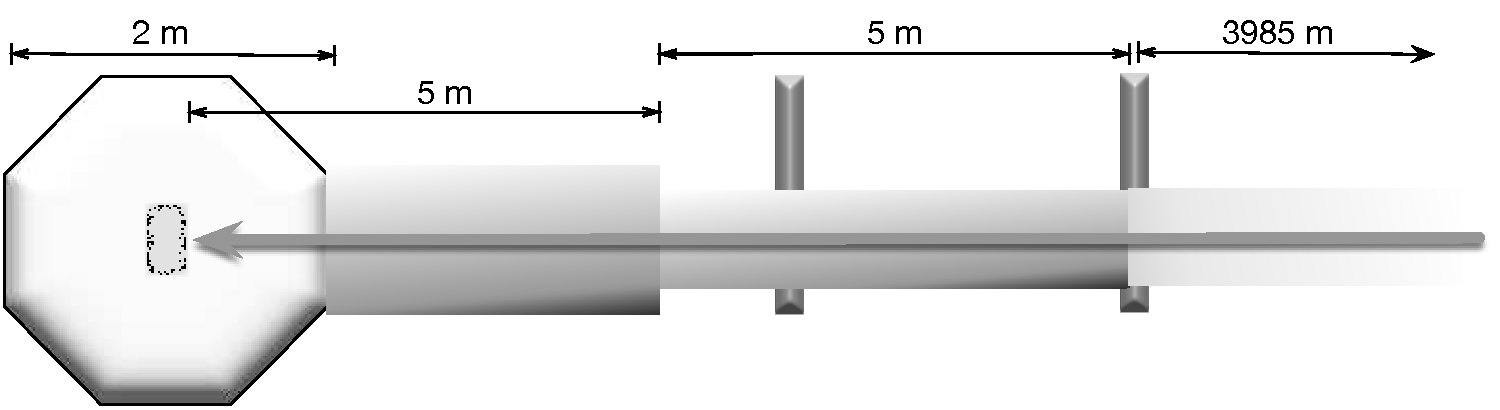
\includegraphics[width=\columnwidth]{Figures/ETM_scatter-BW.pdf}
    \caption{Schematic diagram of a LIGO interferometer mirror and
    surrounding vacuum chambers responsible for backscattered light.}
    \label{fig:ETMscat}
\end{figure}



\subsubsection{Case II: The Test Mass Chambers}
During the operation of the first generation of kilometer scale interferometers,
it became clear that the scattered light from the test mass mirrors was not
all concentrated into small angles (as predicted by theory for super-polished
optics). To calculate the total power scattered into wide angles, one can use the
equivalent of Fermi's 'Golden Rule'\,\cite{Weiss:Scatter97} for optical scattering:
\begin{equation}
\frac{dP}{P} = \left( \frac{4 \pi \sigma}{\lambda} \right)^2
\label{eq:GoldenRule}
\end{equation}
where $\sigma$ is the RMS surface roughness, and $\lambda$ is the
laser wavelength. Combining the measurement result from
Figure~\ref{fig:PhaseMap} with \eqref{eq:GoldenRule}, we can see that the power radiated into
angles ($\theta_{scat} = \lambda / d_{rough}$) greater than 1\,degree should be
less than 0.1\,ppm. This underestimates the true number by
at least 2 orders of magnitude.

Based on cavity ringdown and resonant reflectivity tests (cf.~\cite{Isogai2013}),
the round trip (arm cavity) loss in the initial LIGO interferometers ranged from
$\sim$60--140\,ppm. For two of the Advanced LIGO interferometers, the loss
is in the $\sim$80--120\,ppm range. Wide angle, \textit{in situ},
measurements (using calibrated photodetectors and CCD cameras) show
that the total loss for $\theta_{scat} \gtrsim 1\deg$ is $\sim$\,15\,ppm.
However, it is not at all clear that the angular distribution in that
range is that of a Lambertian surface. Measurements taken at angles of
$\sim$ (0.5 m)/(4000 m) $\approx 0.1$\,mrad show a large azimuthal dependence
(i.e. the BSDF is not symmetric around the beam axis).
Images
such as the one in Figure\,\ref{fig:2kETMy}, implicate point-like structures.
Repeated cleaning of the surface using various techniques reveals a largely
unchanging pattern, implying that the points are defects in the dielectric
mirror coatings, rather than surface contaminants. Although the details of the
story are still being investigated, it seems possible that the defects
are due to artifacts of the ion beam sputtering process as well as
crystal formation in the amorphous thin films during the
post-deposition annealing.

%\subsubsection{Case III: Backscatter from the Dark Port}
\paragraph{Backscatter from the Dark Port}



\begin{figure}[h]
  \centering
    \includegraphics[width=\columnwidth]{Figures/Cheryl-2ketmy.pdf}
    \caption{Image of an initial LIGO test mass during normal operation. The large blob near the top of the image is due to a low power diagnostic beam. The 'starry night' of points are believed to be due to point defects in the high reflection coating and contribute to small and large angle scattering. Photo credit: Cheryl Vorvick (LHO)}
    \label{fig:2kETMy}
\end{figure}


\begin{figure}
    \centering
    \subfloat[Phase Map]{{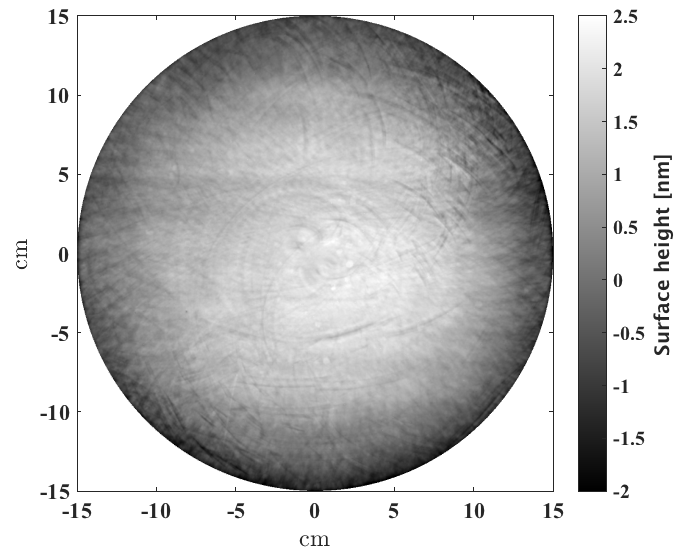
\includegraphics[width=6cm]{Figures/ETMphasemap.png} }}
    \qquad
    \subfloat[Surf PSD]{{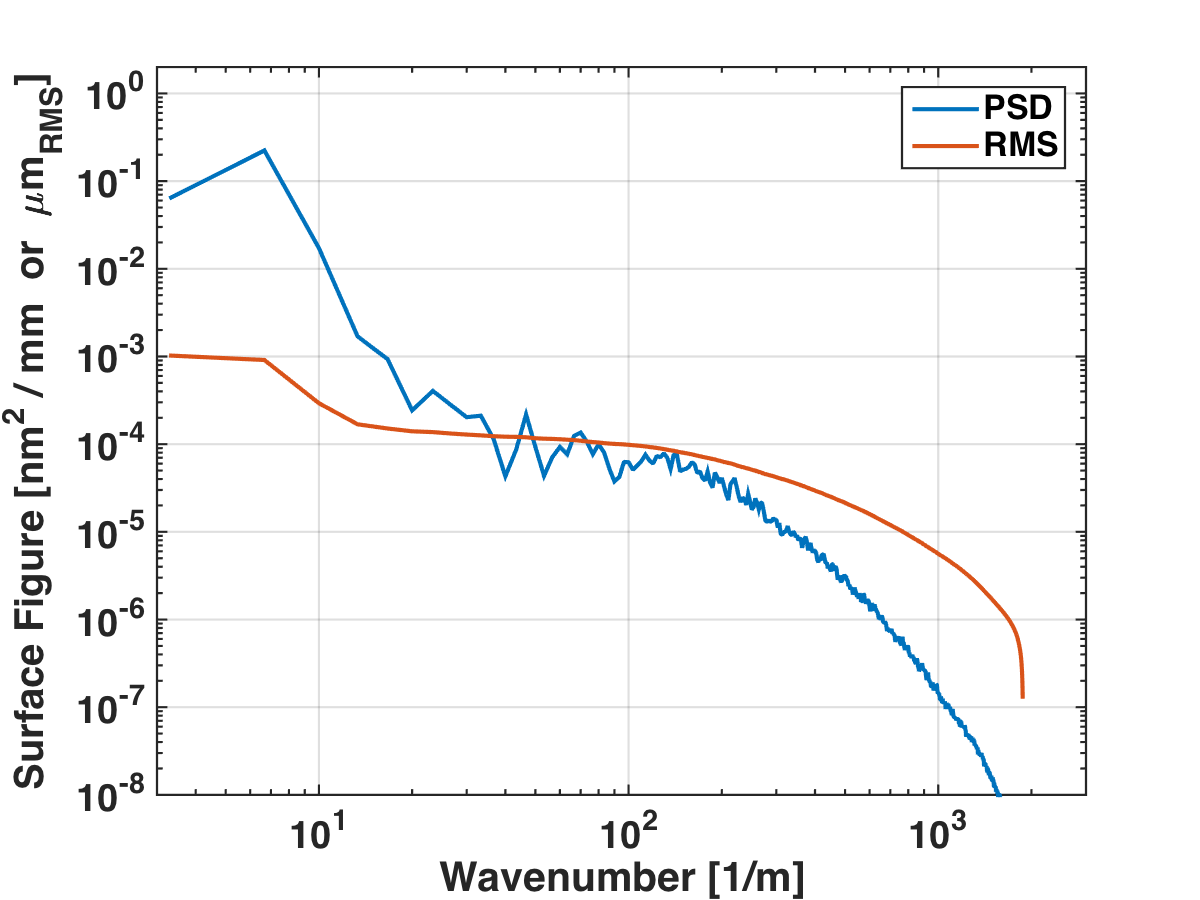
\includegraphics[width=5.5cm]{Figures/ETMpsd.png} }}
    \caption{(left) Surface figure of an uncoated LIGO mirror (ETM07) with the
      spherical curvature and tilt subtracted. The ripple pattern at a radius
      of 3\,--\,15\,cm from the center is due to the planetary coating technique.
      (right) 1D power spectrum of surface. Also
      plotted is the RMS surface roughness integrated from high to low
      spatial frequency.}
    \label{fig:PhaseMap}
\end{figure}

%\subsubsection{Case IV: Backscatter from the Bright Port}
